\RequirePackage[2020-02-02]{latexrelease}
\documentclass{SSBT-BE}
\usepackage[utf8]{inputenc}
\usepackage{makeidx}
\usepackage{amssymb}
\usepackage{amsmath}
\usepackage{graphics}
\usepackage{subfigure}
\usepackage{multirow}
\usepackage{tabularx}
\usepackage{caption}
\usepackage{subcaption}
\usepackage{float}
\usepackage{%
  babel,
  algorithmic,
  algorithm,
  caption
}

\usepackage{url}
\usepackage[breaklinks=true]{hyperref}

\usepackage[intoc]{nomencl}
\renewcommand{\nomname}{Abbreviations}
\makenomenclature

\makeindex

\begin{document}

\title{E-Buddy for Rescued Child Labour}
\author{Sunidhi Jagdish Chavan\\Darshana Kamalakant Ingale \\Lina Shamkant Baviskar \\ Rekha Raju Mahajan }

\dept{Department of Computer Engineering}
\supervisor{Prof. Akash D. Waghmare}
\submitdate{2022 - 2023}
\degree{Bachelor of Engineering}
\specialization{Computer Engineering}
\type{Minor Project}
%\type{Seminar}
\hod{Dr. Manoj E. Patil}



\beforepreface
\prefacesection{Acknowledgement}
We would like to express our deep gratitude and sincere thanks to all who helped us in completing this project report successfully. Many thanks to almighty God who gave us the strength to do this. Our sincere thanks to Principal Prof. Dr. Girish. K. Patnaik for providing the facilities to complete this Project report. We would like to express our gratitude and appreciation to all those who gave us the possibility to complete this report. A special thanks to Prof. Dr. Manoj E. Patil, Head of the Department, whose help, stimulating suggestions and encouragement, helped us in writing this report. We would also like to thank Prof. Akash D. Waghamare, Project Guide, who has given his full effort in guiding us and achieving the goal as well as his encouragement to maintain the progress in track. I am also sincerely thankful to Mrs. Shital Patil, Incharge of Project, for her valuable suggestions and guidance. We would also like to appreciate the guidance given by other supervisor that has improved our presentation skills by their comments and tips. Last but not the least, we are extremely thankful to our parents and friends without whom it could not reach its successful completion.

\begin{flushright} 
Sunidhi Jagdish Chavan 
 
 Darshana Kamalakant Ingale
 
 Lina Shamkant Baviskar
 
 Rekha Raju Mahajan
 \end{flushright}

\printnomenclature




\newpage
\afterpreface
\listoffigures
\listoftables
%\input{glossary}
\clearpage
\pagenumbering{arabic}
\pagestyle{plain}


\prefacesection{Abstract}
Children are employed due to social obligation, or loans and debts made by the families. Usually, children are forced to employ their families in brick kilns, stone and quarries, and agricultural sectors.

The children of the migrant workers and those that belong to the marginalized sections and Dalits in the society are pledged to work in small production houses and factories in the urban areas. Child Labourers on the bond are usually subjected to physical, emotional, mental, and sexual abuse, even leading to death.

In this regard, the approach will be for user to capture images and provide further information of the witnessed act of child labour. After scrutinization the filtered data will be provided to the concerned authorities. This will add impetus to establish a child labour free nation, E-Buddy for rescued child labour website will provide effective enforcement for no child labour. Which will be reducing the incidence of child labour and helpful for government of India.

\acknowledge

\chapter{Introduction}
Child labour is a global phenomenon. Employment of children in any manual work is known as child labour. According to the Child labour (prohibition and regulation) act, 1986. A child is a person who has not yet attained the age of fourteen years. In this tender age where a child is expected to grow , enjoy its childhood to the fullest , seek condition, gain a strong value system goes to work to earn a living either for himself/herself and for their family. Child labour also deprives children of their dignity, potential and their childhood. Children working below the age of 14 years are not able to develop mentally, socially, physically and morally.

The organization of this Chapter is as follows. Section 1.1 describes Background of the project. Motivation of the project is represented in Section 1.2 Section 1.3 represents Problem statement of the project. Scope of the project is described in Section 1.4. Section 1.5 describes Objective of the project. Section 1.6 describes the selection of life cycle model. Section 1.7 shows the organization of report and finally, the Summary is described in 1.8 Section.

\section{Background}
Despite rates of child labour declining over the last few years, children are still being used in some severe forms of child labour such as bonded labour, child soldiers, and trafficking. Across India child labourers can be found in a variety of industries: in brick kilns, carpet weaving, garment making, domestic service, food and refreshment services (such as tea stalls), agriculture, fisheries and mining. Children are also at risk of various other forms of exploitation including sexual exploitation and production of child pornography, including online.

Not solving this problem can result in extreme bodily and mental harm, and even death of the victim. It can lead to slavery and sexual or economic exploitation. And in nearly every case, it cuts children off from schooling and health care, restricting their fundamental rights and threatening their futures.              


\section{Motivation}
Children on the move risk being forced into work or even trafficked – subjected to violence, abuse and other human rights violations. Children may be driven into work for various reasons. Most often, child labour occurs when families face financial challenges or uncertainty – whether due to poverty, sudden illness of a caregiver, or job loss of a primary wage earner. Hence,the project aims to reduce child labour and provide them with necessary resources so as the suffering children can lead a normal and peaceful life.

\section{Problem Definition}
Children are the future of nation and subjecting children to extreme labour causes bodily and mental harm of the child,which in long run threatens the future and development of the child and nation furthermore. Such crimes cannot be reduced unless they are brought in attention of the concerned authorities. To amend the situation of child labour, it is necessary for such crimes to come into attention. And to identify and then furthermore save the children from such labour,a system has to be developed.


\section{Scope}
The proposed system has a very minimal footprint on the overall system and can be easily accessed in the existing system. It will accept name, description and image of victim in a particular format, process and scrutinize it to check whether the activities involved fit into the specified occupations in The (Prohibition and Regulation) Child Labour Act,1986.\\ Following are the functions which this system is expected to do:
\begin{itemize}
\item The project will provide an efficient platform for the detection of child labour
\end{itemize}


\section{Objectives}
The proposed system is built to give a helping hand for prohibiting child labour and provide resources for regulating the lives of children who suffer.\\
The objectives of this project are as follows:
\begin{itemize}
\item To reveal the reasons and consequences of child labour.
\item To eradicate any kind of child abuse in the form of employment and prohibit maltreatment of children in workplace.
\end{itemize}


\section{Selection of Life cycle model for development}
The software development life cycle model selected for this project is the Waterfall Model. Waterfall approach was the first SDLC (Software Development Life Cycle) Model to be widely used in software engineering to ensure success of the project. It was developed by Winston W. Royce in 1970. In ”The Waterfall” approach, the whole process of software development is divided into separate phases, typically the outcome of one phase acts as the input for the next phase sequentially. All the phases are cascaded to each other in which progress is seen as flowing steadily downwards (like a waterfall) through the phases. Re-quirements for this project are well documented and fixed.

\begin{figure}[H]
    \centering
    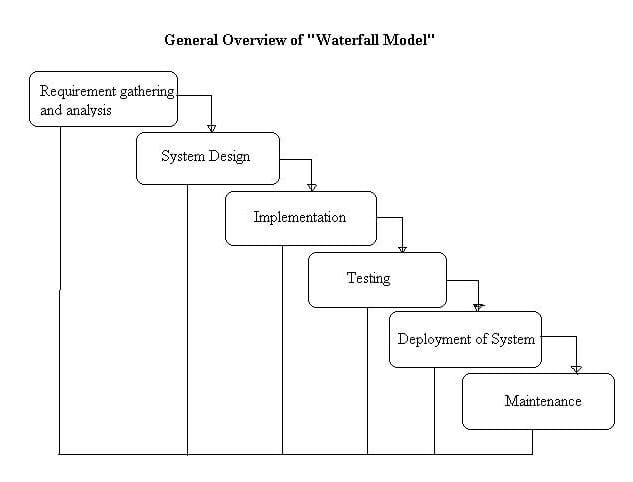
\includegraphics[scale=0.68]{introduction/Waterfall Model.jpg}
    \caption{ Waterfall Modell}
    \label{fig:my_label}
\end{figure}

Waterfall Model is best suited model for this project.
\begin{itemize}
\item Because requirements are easily understandable and defined
\item We can define requirements in early stage of development
\item User involvement in all phases is not necessary
\item Limited user’s participation
\end{itemize}
    
\section{Organization of Report}
\hspace{1cm}Chapter 1: entitled as Introduction describes the details about Background, Problem     Definition, Scope and Objective of the project, Identification of Software Development Process Model and Organization of report. \\

\hspace{0.5cm}Chapter 2: entitled as Project Planning and Management consists of details about the Feasibility Study, Risk Analysis, Project Scheduling, Effort Allocation and Cost Estimation of the project. \\

\hspace{0.5cm}Chapter 3: entitled as Analysis describes in detail, the Requirement Collection and Identification, H/w and S/w Requirements, Functional and Non-Functional Requirements and a Software Requirements Specification(SRS). \\

\hspace{0.5cm}Chapter 4: includes design about System Architecture, Data Flow Diagram and various UML Diagrams. \\
 


\section{Summary}
As mentioned in above sections, this project aims at building an ebuddy for rescuing child labour. The scopes, objective, etc. are as mentioned above. In the next chapter, project planning and management will be discussed.

\chapter{Project Planning And Management}
Project planning is a procedural step in project management. It is the practice of initiating, planning, executing, controlling and closing the work team to achieve specific goals. Project planning and management is important because it ensures that the right people do the right things, at the right time.  It also ensures the proper project lifecycle.

The organization of this chapter is as below. Section 2.1 shows the Feasibility Study of the project. Risk Analysis of the project is represented in Section 2.2 and Project Scheduling is described in Section 2.3. Section 2.4 and 2.5 describe the Effort Allocation and Cost Estimation respectively. The Summary is mentioned in Section 2.6.

\section{Feasibility Study}

A feasibility study is an assessment of the practicality of a proposed project or system. A feasibility study aims to objectively and rationally uncover the strengths and weaknesses of an existing business or proposed venture, opportunities and threats present in the natural environment, the resources required to carry through, and ultimately the prospects for success. In its simplest terms, the two criteria to judge feasibility are cost required and value to be attained. A well-designed feasibility study should provide a historical background of the business or project, a description of the product or service, accounting statements, details of the operations and management, marketing research and policies, financial data, legal requirements and tax obligations. Generally, feasibility studies precede technical development and project implementation.

A feasibility study evaluates the project’s potential for success; therefore, perceived objectivity is an important factor in the credibility of the study for potential investors and lending institutions. It must therefore be conducted with an objective, unbiased approach  to provide information upon which decisions can be based. Taking into consideration the technical, operational and economic feasibility as below, the project can be anticipated as feasible overall. There are few types of feasibility that exists. So, developers should take care of these feasibility and take them into consideration:


\subsection{Technical Feasibility}
This assessment is based on an outline design of system requirements, to determine whether the company has the technical expertise to handle completion of the project. At this level, the concern is whether the proposal is both technically and legally feasible (assuming moderate cost). It is an evaluation of the hardware and software and how it meets the need of the proposed system.

This project is built upon Jupyter Notebook, a simple Web-Application or CLI with Python as the programming language and can be easily hosted on cloud server. Also all the other technologies used are capable of building such a project and serve as well as maintain it for longer period of time. All the required hardware and software are easily available in the market. Hence the project is technically feasible.




\subsection{Operational Feasibility}
Operational feasibility is the measure of how well a proposed system solves the problems, and takes advantage of the opportunities identified during scope definition and how it satisfies  the requirements identified in the requirements analysis phase of system development.

The operational feasibility assessment focuses on the degree to which the proposed development project fits in with the existing business environment and objectives with regard to development schedule, delivery date, corporate culture and existing business processes. The application is operationally feasible since it is build with the idea for integration with various existing applications and systems.


\subsection{Economical Feasibility}
Describes how much time is available to build the new system, when it can be built, whether it interferes with normal business operations, type and amount of resources required, dependencies, and developmental procedures with company revenue prospectus.

As the necessary hardware and the software are easily available in the market at low cost, the initial investment is the only cost incurred and does not need further enhancement. Hence it is economically feasible.


\section{Risk Analysis}
Risk Analysis and Management is a key project management practice to ensure that the least number of surprises occur while your project is underway. While we can never predict the future with certainty, we can apply a simple and streamlined risk management process to predict the uncertainties in the projects and minimize the occurrence or impact of these uncertainties.

This project has a very slight window for experiencing failures not in technical aspects but those functionalities involving real life interaction might be affected. 

\section{Project Scheduling}
Generally, project scheduling can be stated as the estimated time required for any project from its time of beginning to the end of the project. In detail, for every task, there is a deadline because all the tasks for the completion of project are planned earlier. So that, each task is scheduled to certain time limit.   15 In short, in project management, listing of projects milestones, activities and all from starting to end date, are considered in the project scheduling. A schedule is generally used in the project planning and management of the project with some kind of attributes as budget, task allocation and duration, resource allocation and all.
 \begin{table}[H]
     \centering
     \begin{tabular}{c|c}
         
         \begin{tabularx}{1\textwidth} { 
  | >{\raggedright\arraybackslash}X 
  | >{\raggedright\arraybackslash}X 
  | >{\raggedright\arraybackslash}X|}
 \hline
  Task & Start Date & End Date \\
 \hline
 Selection of title &26 Aug 2022&29 Aug 2022\\
\hline
  Gathering information  &30 Aug 2022&19 Sep 2022\\
\hline
 Project discussion &20 Sep 2022&30 Sep 2022 \\
\hline
  Planning/ requirement gathering and  analysis  &3 Oct 2022&7 Oct 2022 \\
\hline
 Design &7 Oct 2022&14 Oct 2022 \\
\hline
Knowledge and Gathering &17 Oct 2022&2 Dec 2022\\
\hline
Development Phase &5 Dec 2022&11 Jan 2023\\
\hline
Testing &12 Jan 2023&17 Jan 2023\\
\hline
Documentation &26 Aug 2022&15 Mar 2023\\
\hline


\end{tabularx} 
     \end{tabular}
     \caption{Task Scheduling for the project}
     \label{tab:my_label}
 \end{table}
 \begin{figure}[H]
    \centering
    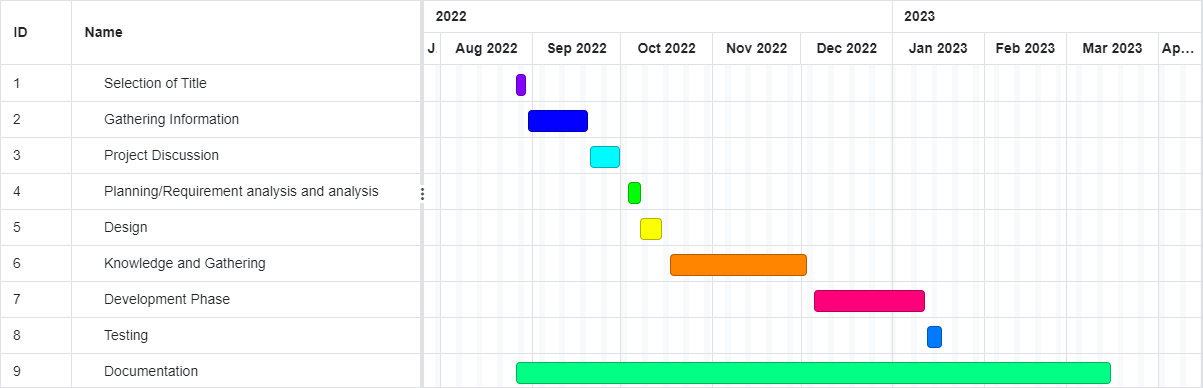
\includegraphics[scale=0.42]{design/Gantt fin.png}
    \caption{Gantt Chart}
    \label{fig:my_label}
\end{figure}    



\section{Effort Allocation}
Effort Allocation is necessary so every team member can give its best to the project. Project was divided into smaller module and task form, for simplification and easy understanding of project overall. Some modules include every team associate’s presence to take advantage of team decision taking skills, and some task include some individual member to work on it with precision. We divided the project into 6 modules.
\begin{itemize}

\item 1.	Gathering of Information
\item 2.	Planning/Requirement Analysis
\item 3.    Selection of Life Cycle
\item 4.	Planning and Management
\item 5.	Analysis & Design UML
\end{itemize}



\begin{table}[H]
    \centering
    \begin{tabular}{c|c}
         \begin{tabularx}{1\textwidth} { 
  | >{\raggedright\arraybackslash}X 
  | >{\centering\arraybackslash}X
  | >{\centering\arraybackslash}X
  | >{\centering\arraybackslash}X
  |>{\centering\arraybackslash}X | }
 \hline
 & Sunidhi & Darshana & Rekha & Lina \\
 \hline
Gathering of information &\checkmark &\checkmark &\checkmark &\checkmark\\
\hline
planning / requirement analysis  &&\checkmark&\checkmark&\\
\hline
 selection of life cycle   &\checkmark&& &\checkmark \\
\hline
planning and management &\checkmark&\checkmark&& \\
\hline
analysis and design &&&\checkmark&\checkmark \\
\hline

\end{tabularx} 
    \end{tabular}
    \caption{Effort Allocation }
    \label{tab:my_label}
\end{table}




\section{Cost Estimation}
Cost Estimation is an important phase for any project. It predicts if the project investment is adequate or there will shortage of capital. It presents the total cost required for development of project. Cost Estimation should be done before initiating the development to prevent loss of efforts and project failure during development. For estimation of cost for this project, we need to consider the server costs for deployment, although the cost is extremely variable since it is dependent on real-time usage.
The cost for a machine learning project is generally calculated in three components i.e. data cost, research cost and production cost. Since our project has the required dataset already available, the data cost for the project is zero. The research cost is dependent on the number of people involved in the project for the amount of time required for the project. Assuming the cost for each person who does research to be Rs. 20000 per month, if 4 people work for a timeline of 6 months, the research cost will be\\

Research Cost = 4 people x 6 months x Rs. 20000\\
= Rs. 4,80,000\\

According to the Google Cloud Calculator, the cost for deploying an E2 compute engine with Windows as operation system, 4 vCPU’s and 16 GB RAM is Rs. 7000 per month. If the deployment is to be done for 12 months, the production cost will be
 
Production Cost = 12 months x Rs. 7000\\
= Rs. 84,000

Hence the total cost of the project can be calculated as

Total Cost = Research Cost + Production Cost\\
= Rs. 4,80,000 + Rs. 84,000\\
Total Cost = Rs. 5,64,000


\section{Summary}
The project, is hence found to be feasible since there is a balance of resources required and the cost incurred. Also the project helps the government to identify crime like child labour. The project will be able to easily integrate with other required systems.

%\chapter{Key Management}
\label{CH-Key Management}
%\input{./key/gkp}

\chapter{Analysis}

The development of computer-based information system includes the system analysis phase which produces or enhances the data model which itself is to creating or enhancing a database.   There are a number of different approaches to system analysis.    The analysis is the process which is used to analyze, refine and scrutinize the gathered information of entities in order to make consistence and unambiguous information. Analysis activity provides a graphical view of the entire System. System Analysis is the process of gathering and interpreting facts, diagnosing problems and using the facts to improve the system. System analysis chapter will show overall system analysis of the concept, description of the system, meaning of the system. System analysis is the study of sets of interacting entities, including computer system analysis.

The organization of this Chapter is as follows. Section 3.1 represents Requirement Collection and Identification. Software Requirement and Specification are described in the Section
3.2. Section 3.3 describes summary of the chapter.

\section{Requirement Collection and Identification}
Requirement collection is the process which is used to gather, analyze, and documentation and reviews the requirements. Requirements describe what the system will do in place of how. In practical application, most projects will involve some combination of these various methods in order to collect a full set of useful requirements. Requirements collection is initiated when the project need is first identified and the project “solution” is to be proposed. Requirements refinement continues after the project is “selected” and as the scope is defined, aligned and approved.

The system will require only images of the road to be analysed which will be uploaded by user either through the web-application or CLI.

\section{Software Requirements Specifications (SRS)}
Software Specification will provide a broad understanding of the requirement specification of this system. Also, understand features of this system along with the requirements. Software Requirement Specification documents guide the developers in the development process and it will help to reduce the ambiguity of the requirements provided by the end-user. It’s used to provide critical information to multiple teams — development, quality assurance, operations, and maintenance. This keeps everyone on the same page.
\subsection{Product Feature}
The product features are high level attributes of a software or product such as software performance, user-friendly interface, security portability, etc. These attributes are defined according to the product, in this case, a software product.\\
They are as follows:
\begin{itemize}
\item The user will be able to upload the name, description and image of the child labour.
\item The user will be able to view the results of submitted images.
\item Our websites enables retailers to set up online shops, customers to browse through the shops, and system administrator to approve and reject requests for new shops and maintain lists of shop categories.
\item The user will be provided with gift cards for their contribution towards the welfare of children.
\end{itemize}

\subsection{Operating Environment}
The software will operate within the following environment:
\begin{itemize}
    \item  Operating System: Windows 7 or later/Linux/MacOS
    \item Java environment required.
    \item Any system with at least 2GB RAM
    \item System with processor Intel CORE i3 or later
\end{itemize}

\subsection{Assumption}

\begin{itemize}
\item It is assumed that the web portal will load and render correctly and as expected on the operating machine.
\item It is assumed that the user will have a working internet connection with sufficient internet speed.
\item It is assumed that the user is able to either upload images through web interface or CLI.
\item It is assumed that the user will upload the images within the given specifications.
\end{itemize}


\subsection{Functional Requirements}
Functional requirements are the functions which are expected from the software or platform. Functional requirements along with requirement analysis help identify missing requirements. They help clearly define the expected system service and behavior.\\ Functional requirements are as follows:
\begin{itemize}
    \item To be able to upload the images through the web interface and command line interface.
    \item To be able to view the results of analysis through web as well as command line interface.
\end{itemize}

\subsection{Non-Functional Requirements}
Non-functional Requirement is mostly quality requirement. That stipulates how well the portal does, what it has to do. Other than functional requirements in practice, this would entail detail analysis of issues such as availability, security, usability and maintainability.\\
Non-functional requirements are as follows:
\begin{itemize}
    \item The processing system is fast enough to reduce the existing delays.
    \item The interface should be simple and minimal.
    \item The results should be comprehensive and detailed. 
\end{itemize} 

\subsection{External Interfaces}

\begin{itemize}
 \item[$\blacksquare$] {\large User interface}\\
The proposed system has several options for users to interact with. Following are the user interfaces available:
 \item Web-application (GUI)
 \item Command Line Interface (Terminal based interface)\\
The web application will be available so that the users will be able to upload images through a simple GUI and the CLI will be available so that the user will be able to integrate it with other systems easily.

\item[$\blacksquare$] {\large Software interface}\\
The only software interface required for this project is the Application Programming Interface with the Jupyter Notebook which will then process the images. This software interface will run on local server along with the Jupyter server.
\end{itemize}

\section{Summary}
In the chapter, Analysis was presented which included the hardware and software require- ments, functional and non-functional requirements and the software requirements specifi- cation(SRS) as well. In the next chapter, Design is described along with various UML diagrams.

\chapter{Design}
Design is the activity to design and model the various component of software system. The system design provides the understanding and procedural details necessary for implementing the system. Design is helpful for a better understanding of the project. It contains the UML diagrams, data flow diagrams. UML is a modeling language which is used to document the object-oriented analysis and design.

The organization of this Chapter is as follows. Section 4.1 describes the system architecture of the project. DFD of the project are represented in Section 4.2. Section 4.3 represents UML Diagrams (Use case, Class, Sequence, Component, Deployment, State chart, Activity diagram, Class Diagram,  Component Diagram,  etc.)  of the project.  Finally,  the Summary is described in last Section 4.4

\section{System Architecture}
Systems Architecture is a generic discipline to handle objects (existing or to be created) called ”systems”, in a way that supports reasoning about the structural properties of these objects. The system architecture is the conceptual model that defines the structure, behavior and more views of a system.

An architecture description is a formal description and representation of a system. It provides broad understanding of the portal. In the system architecture database provide the functionality like get information, select criteria, etc. to users.\\
\newpage
  \begin{figure}
    \centering
    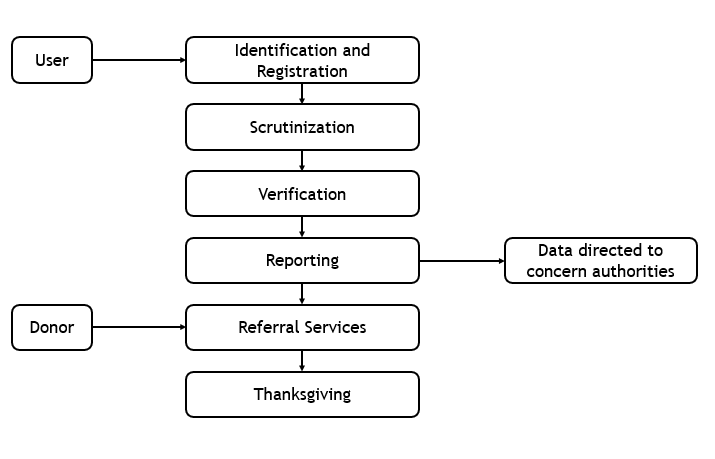
\includegraphics[width= 18cm,scale=0.70]{design/system arch.png}
    \caption{System Architecture }
    \label{fig:my_label}
  \end{figure}
    
    
    
    
\section{Data Flow Diagram}

 A data flow diagram (DFD) is a graphical representation of the ‘flow’ of data through an information system, modelling its process aspects. A DFD is often used as a preliminary step to create an overview of the system, which can later be elaborated. DFDs can also be used for the visualization of data processing (structured design). A DFD shows what kind of information will be input to and output from the system, where the data will come from and go to, and where the data will be stored.

\subsection{Level 0 DFD}
Level 0 contains one input and one output. The system provides information to the user means system is input and the user is output. Figure 4.2 shows Level 0 DFD of project.
\begin{figure}[H]
    \centering
    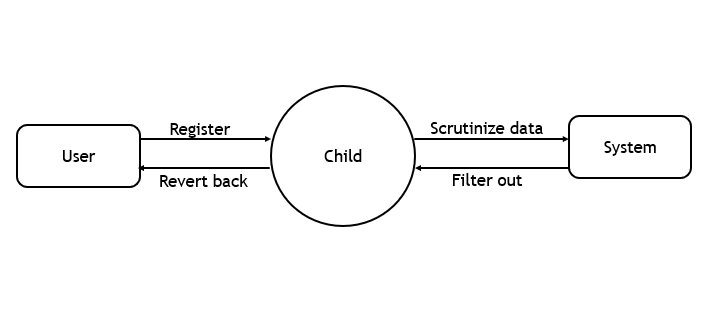
\includegraphics[width = 12cm]{design/0 level DFD.png}
    \caption{ 0 Level Data Flow Diagram}
    \label{fig:my_label}
\end{figure}

\subsection{Level 1 DFD}
A level 1 DFD notates each of the main sub-processes that together form the complete system.   We can think of a level 1 DFD as an “exploded view” of the context diagram. 
Figure 4.3 shows Level 1 DFD of project.
\begin{figure}[H]
    \centering
    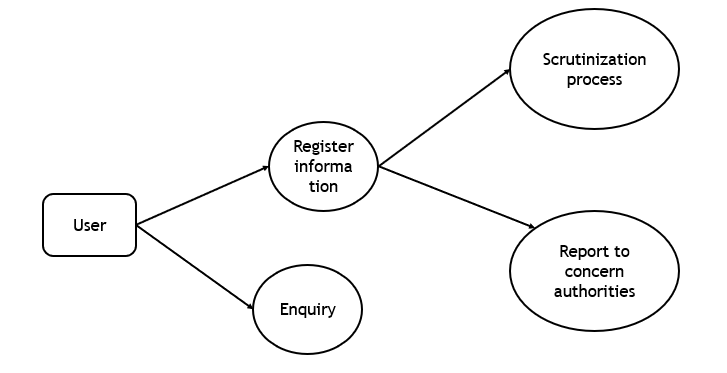
\includegraphics[width = 12cm]{design/1 Level DFD.png}
    \caption{  1 Level Data Flow Diagram }
    \label{fig:my_label}
\end{figure}


\subsection{Level 2 DFD}

A level 2 data flow diagram offers a more detailed look at the processes that make up an information system than a level 1 DFD does. It can be used to plan or record the specific makeup of a system.\\ Figure 4.4 shows Level 2 DFD of project.
\begin{figure}[H]
    \centering
    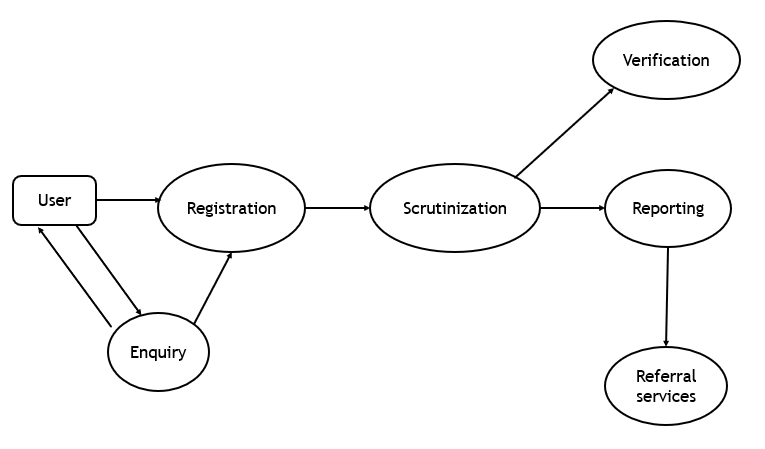
\includegraphics[width=12cm]{design/2 Level DFD.png}
    \caption{2 Level Data Flow Diagram}
    \label{fig:my_label}
\end{figure}

\newpage
\section{UML Diagrams}
A UML diagram is a diagram based on the UML (Unified Modeling Language) with the purpose of visually representing a system along with its main actors, roles, actions, artifacts or classes, in order to better understand, alter, maintain, or document information about the system.

\subsection{Use Case Diagram}
Use case diagram shows the interaction between Use case which represents system functionality and actor which represent the people or system. Fig 4.5 shows use case diagram.
\begin{figure}[H]
    \centering
    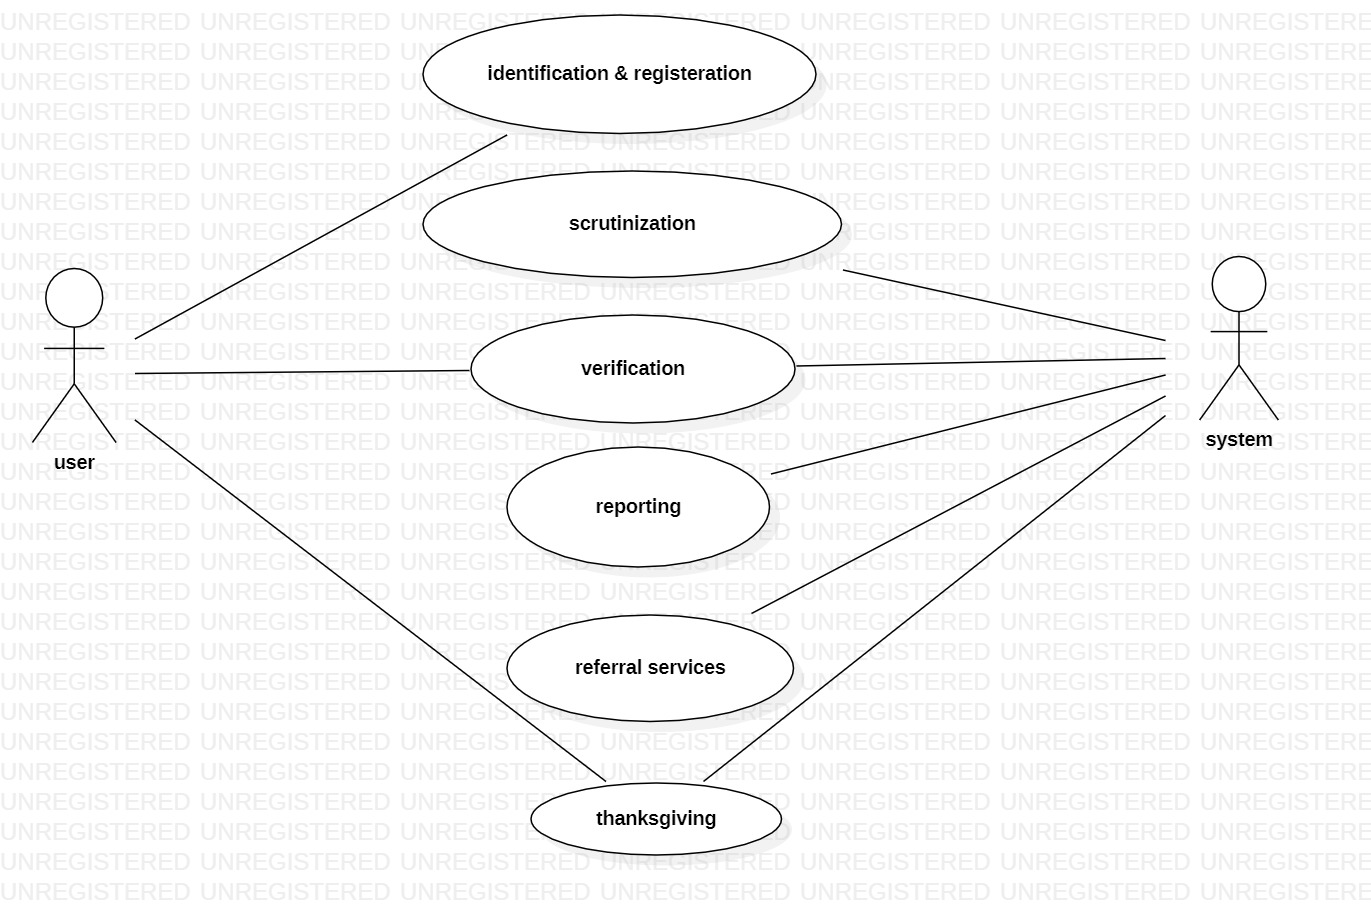
\includegraphics[scale=0.35]{design/usecase.jpg}
    \caption{Use Case Diagram}
    \label{fig:my_label}
\end{figure}


\subsection{Sequence Diagram}

The sequence diagram shows the flow of functionality through Use case. A sequence diagram is a type of interaction diagram because it describes how—and in what order—a group of objects works together. These diagrams are used by software developers and business professionals to understand requirements for a new system or to document an existing process.Fig 4.6 shows sequence diagram.

\begin{figure}[H]
    \centering
    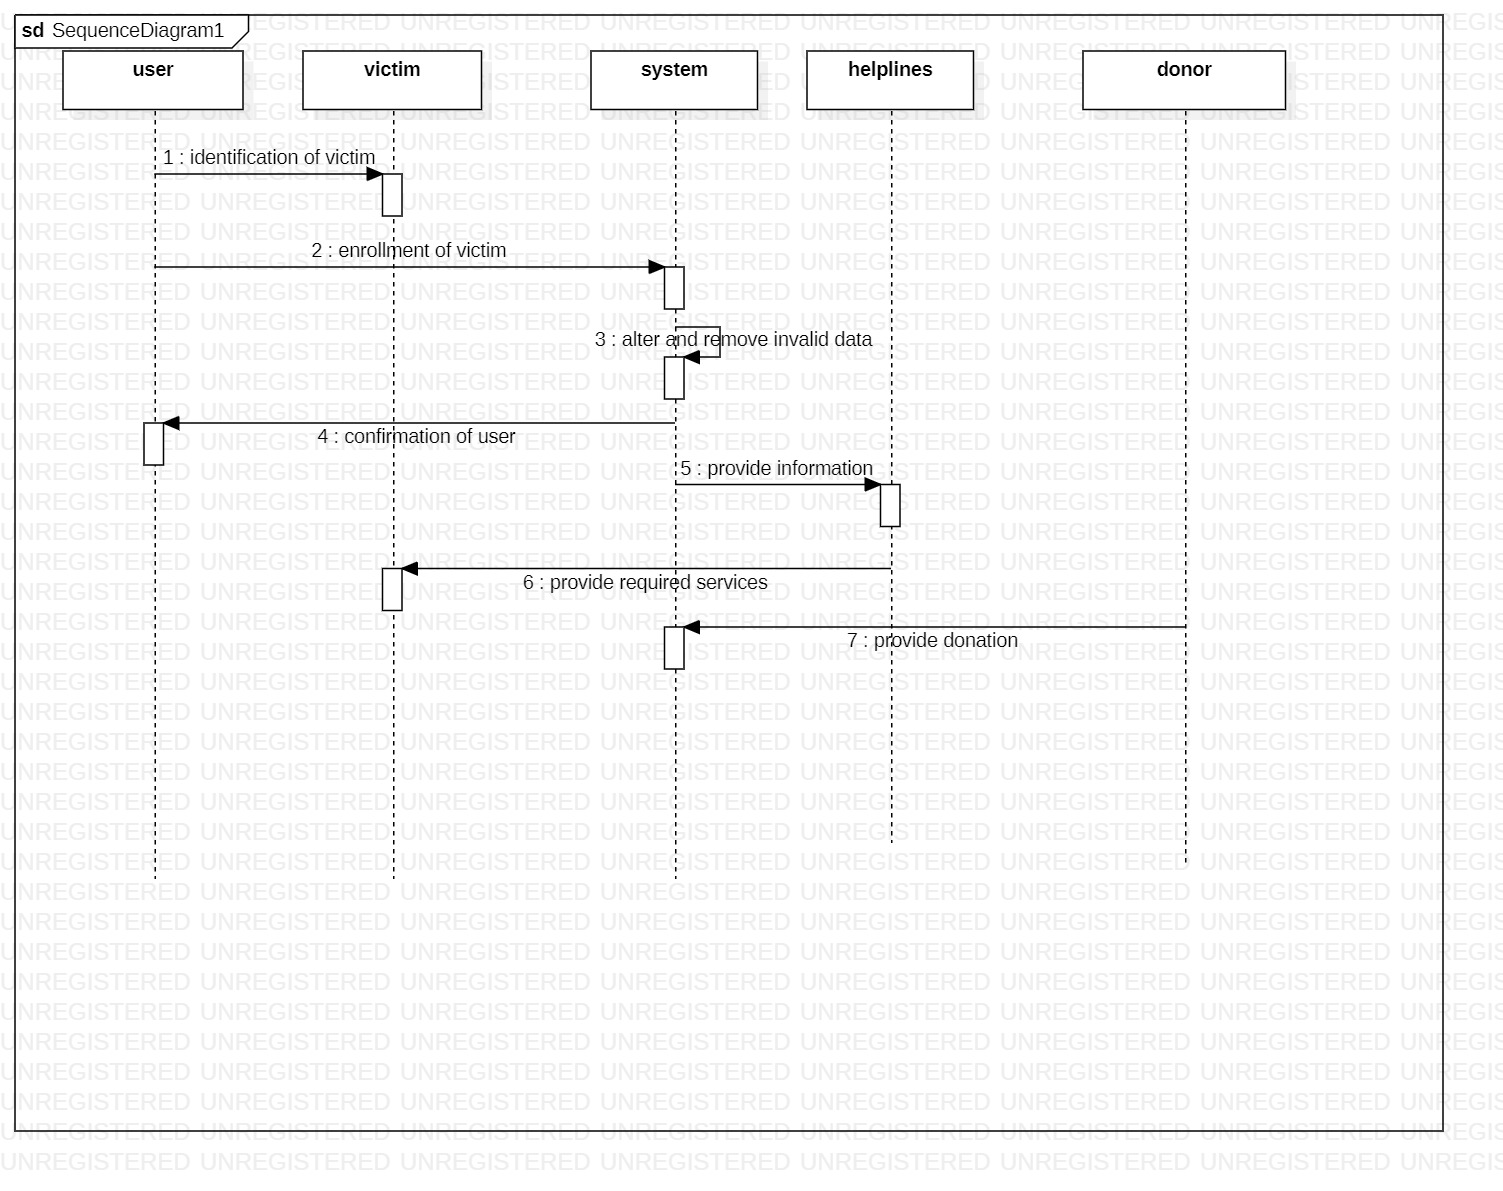
\includegraphics[scale=0.35]{design/SequenceDiagram.jpg}
    \caption{Sequence Diagram}
    \label{fig:my_label}
\end{figure}

\subsection{Collaboration Diagram}
A collaboration diagram, also known as a communication diagram, is an illustration of the relationships and interactions among software objects in the Unified Modeling Language (UML). These diagrams can be used to portray the dynamic behavior of a particular use case and define the role of each object. Fig 4.7 shows collaboration diagram.
\begin{figure}[H]
    \centering
    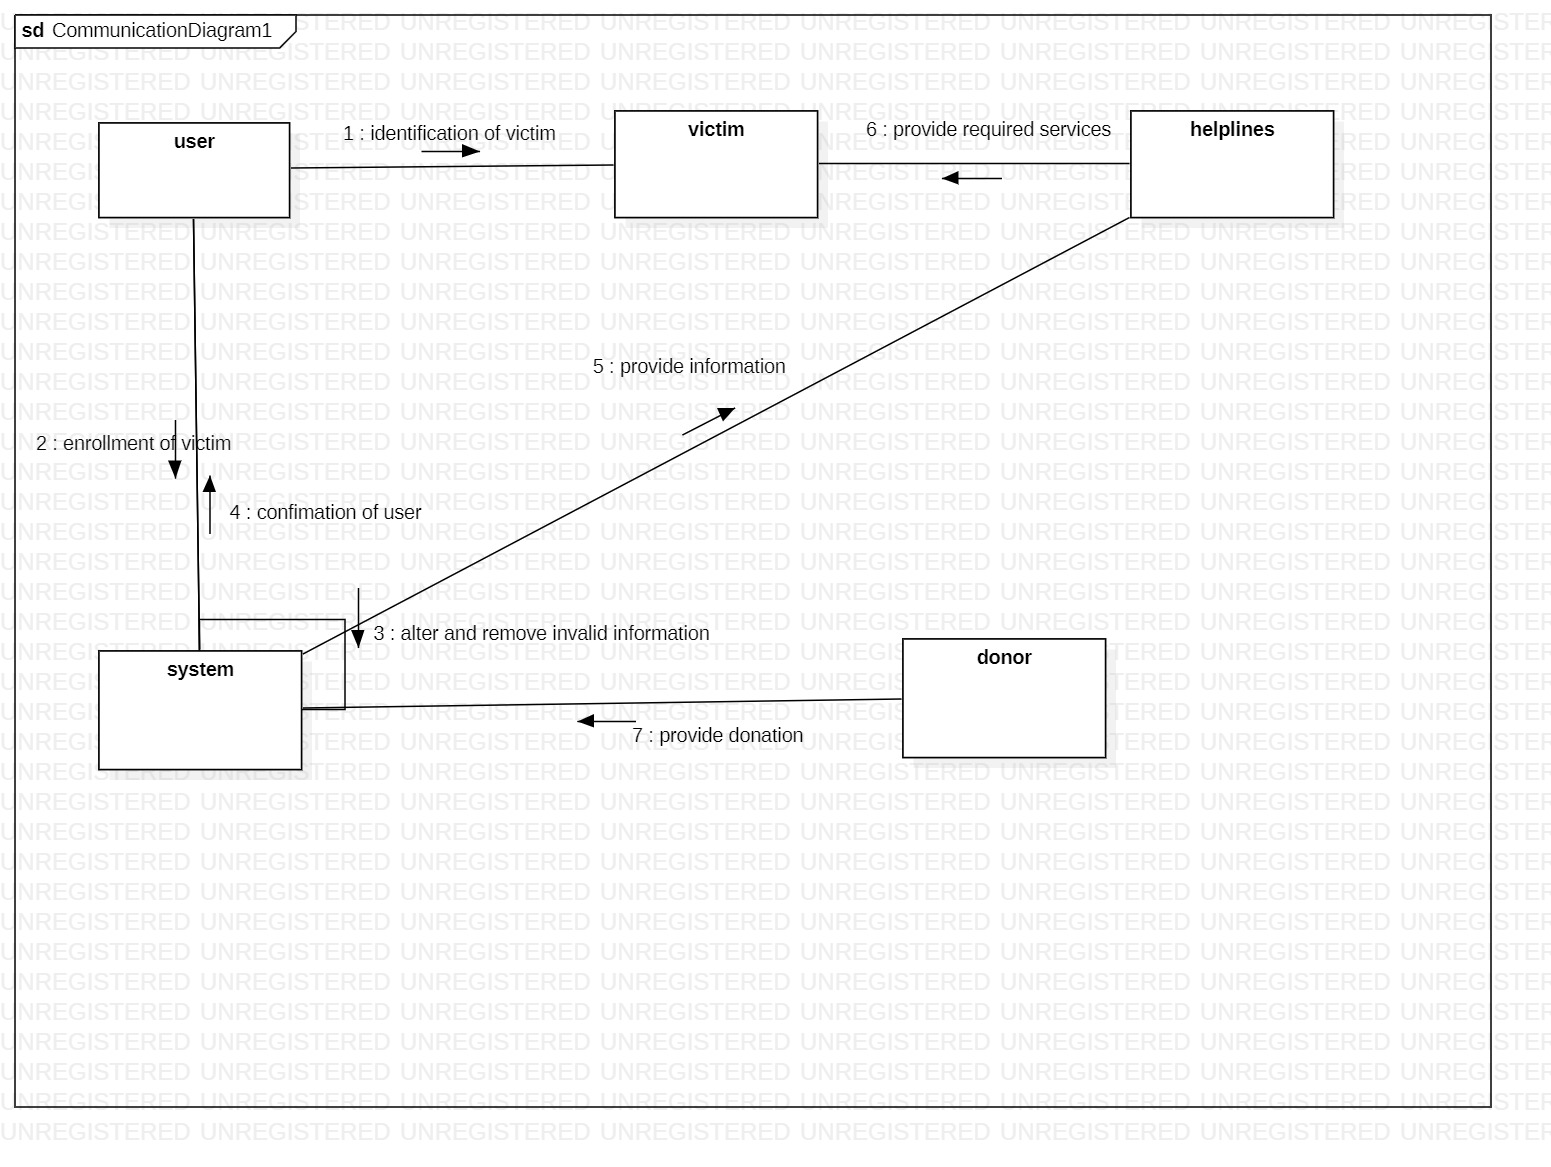
\includegraphics[scale=0.30]{design/CommunicationDiagram.jpg}
    \caption{Collaboration Diagram}
    \label{fig:my_label}
\end{figure}

\subsection{Class Diagram}
The class diagram is the main building block of object-oriented modeling. It is used for general conceptual modeling of the structure of the application, and for detailed modeling translating the models into programming code. Class diagrams can also be used for data modeling. Fig 4.8 shows class diagram.
\begin{figure}[H]
    \centering
    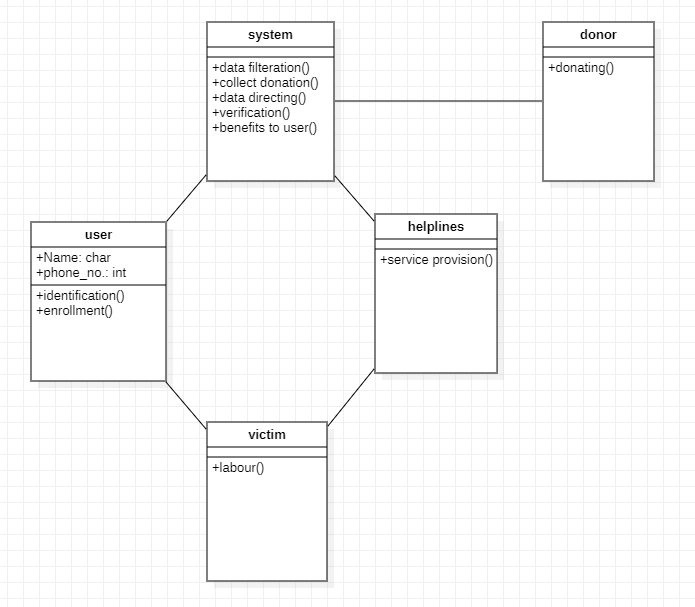
\includegraphics[scale=0.70]{design/ClassDiagram.png}
    \caption{Class Diagram}
    \label{fig:my_label}
\end{figure}

\subsection{Component Diagram}
A component diagram, also known as a UML component diagram, describes the organization and wiring of the physical components in a system. Component diagrams are often drawn to help model implementation details and double-check that every aspect of the system’s required function is covered by planned development.Fig 4.9 shows component diagram.
\begin{figure}[H]
    \centering
    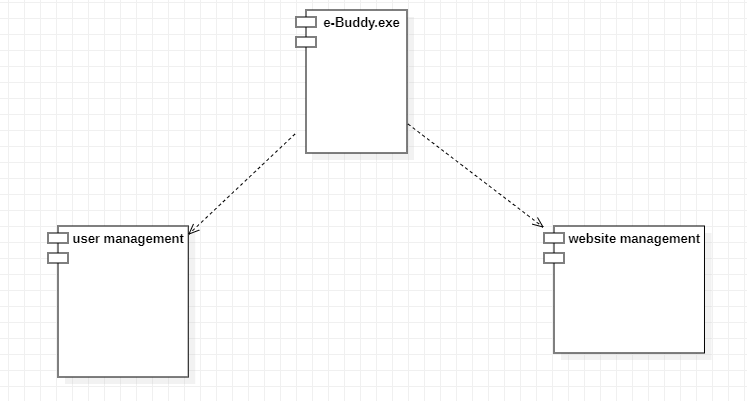
\includegraphics[scale=0.60]{design/ComponentDiagram.png}
    \caption{Component Diagram}
    \label{fig:my_label}
\end{figure}

\subsection{Deployment Diagram}
A deployment diagram is a UML diagram type that shows the execution architecture of a system, including nodes such as hardware or software execution environments, and the middle ware connecting them. Deployment diagrams are typically used to visualize the physical hardware and software of a system. Fig 4.10 shows deployment diagram.
\begin{figure}[H]
    \centering
    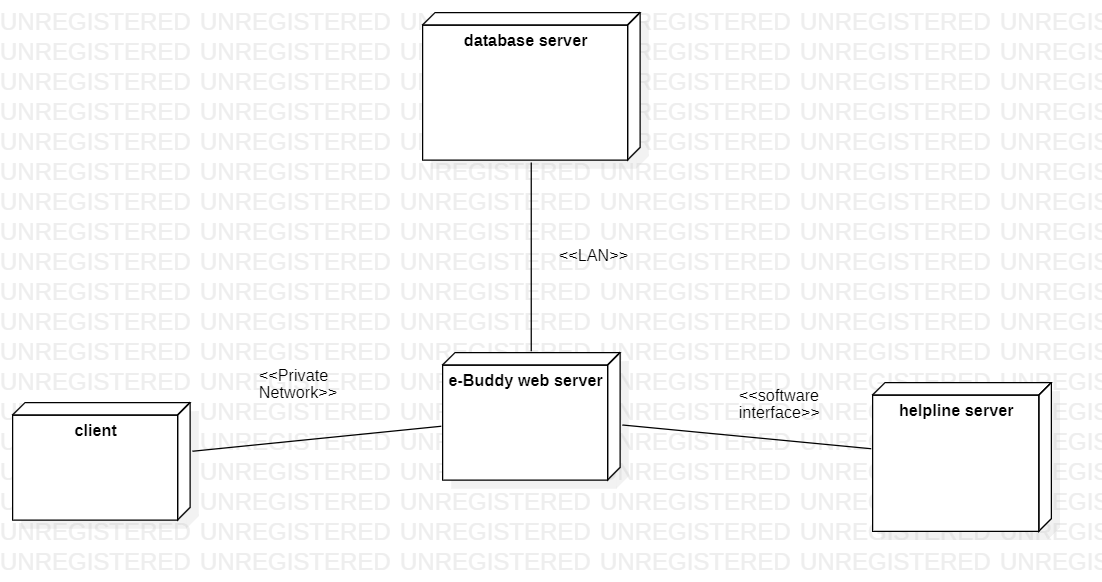
\includegraphics[scale=0.45]{design/DeploymentDiagram1.png}
    \caption{Deployment Diagram}
    \label{fig:my_label}
\end{figure}

\section{Summary}
Detailed design of project has been described in this chapter including the Data Flow Diagrams and the UML Diagram explaining all the design details of the project. Conclusion of the project has been explained in the next chapter. 

\chapter{Implementation}
Important phase in system development is the successful implementation of the new system
design. Implementation includes all those activities that take place to convert from the old
system to the new system. Project Implementation is a practice of executing or carrying
out a project under a certain plan in order to complete this project and produce desired
results. Such a practice encompasses all processes and activities involved in getting the
project plan fulfilled and accomplishing project goals and objectives. 

Section 5.1 describes
the Algorithm. Software and hardware for development is discussed in detail in Section 5.2.
Section 5.3 describes the various Modules in Project

\section {Algorithm/steps}
Following are the steps that should be carried out for the execution of E-buddy.
\begin{itemize}
\item Start: Display Homepage
\item Complaint Form Registration
\item Registered information to be scrutinised
\item Valid scrutinised information forwarded for verification
\item User Verification done using OTP
\item Scratch cards are availed by users through login
\end{itemize}

\section {Software and Hardware for development in detail}
Following are the hardware and software requirements for E-buddy.
\subsection {Hardware Requirements}
\begin{itemize}
\item \textbf {Dedicated PC/Mobile Phone}: For client side user, it is necessary to connect the
server for reaching the website. To visit the website, user required the dedicated PC,laptop, tablet or Mobile phone. Similarly, this PC also required to developer while
developing the System.
\item \textbf {Internet}: For connecting end user to the developed system, Internet is required. Into
the internet nowadays, the 4G speed Internet is best option for reaching the website
because it generates the interest into the user and view contents of the website in a
efficient manner.
\end {itemize}


\subsection {Software Requirements}
\begin{itemize}
\item \textbf {Browser}: This software does not require a particular Operating System to run but
only a web browser and internet connection because it is a web based application.

\item \textbf {XAMPP}: XAMPP is an easy to install distribution to get in the world of Apache.

\item \textbf {MySQL}: MySQL is a relational database management system based on the Structured Query Language,which is the popular language for accessing and managing the records in the database.
\end{itemize}

\section {Summary}
The above chapter describes the coding and implementation of the project. The next chapter
will discuss the testing methodologies of the project.






\chapter{Testing}
Testing is the process of evaluating a system or its component(s) with the intent to find
whether it satisfies the specified requirements or not. In simple words, testing is executing a
system in order to identify any gaps, errors, or missing requirements in contrary to the actual
requirements. Software Testing is a process of verifying and validating whether the program
is performing correctly with no bugs. It is the process of analyzing or operating software
for the purpose of finding bugs. It also helps to identify the defects / aws / errors that
may appear in the application code, which needs to be fixed. Testing not only means fixing
the bug in the code, but also to check whether the program is behaving according to the
given specifications and testing strategies. This Chapter is organized as follows.

Section 6.1
describes Black Box Testing and white Box Testing. Section 6.2 describes Manual Testing
and Automated Testing. Test Cases Identification and Execution describe in Section 6.3.
Finally, summary of the chapter is given in last section

\section{Black Box and White Box Testing}
The following methodologies are used for testing.
\subsection{Black Box Testing}
Black Box testing also known as Behavioral Testing, is a software testing method in which
the internal structure/design/implementation of the item being tested is not known to the
tester. These tests can be functional or non-functional, though usually functional.
This method is named so because the software program, in the eyes of the tester, is like a
black box; inside which one cannot see. This method attempts to find errors in the following categories
\begin{itemize}
\item Incorrect or missing functions
\item Interface errors
\item Errors in data structures or external database access
\item Behaviour or performance errors
\item Initialization and termination errors
\end{itemize}

\subsection{White Box Testing}
White Box Testing is also known as Clear Box Testing, Open Box Testing, Glass Box Testing,
Transparent Box Testing, Code-Based Testing or Structural Testing. It is a software testing
method in which the internal structure, design, implementation of the item being tested is
known to the tester. The tester chooses inputs to exercise paths through the code and determines the appropriate outputs. Programming know-how and implementation knowledge
is essential. White box testing is testing beyond the user interface and into the nitty-gritty
of a system.
This method is named so because the software program, in the eyes of the tester, is like
a white or transparent box; inside which one clearly sees.

\section {Manual and Automated Testing}
Following methodologies are used for testing.
\subsection{Manual Testing}
It is the oldest and most rigorous types of testing it is performed by human sitting in
front of a computer carefully going through applications screens, trying various usage and
input combinations, comparing the results to the expected behavior and recording their
observations about project. There are certain ways of manual testing first of all test cases
are written then they are executed and then report is generated according to test result.
\subsection{Automated Testing}
Automation testing is a Software testing technique to test and compare the actual outcome
with the expected outcome. This can be achieved by writing test scripts or using any
automation testing tool. Test automation is used to automate repetitive tasks and other
testing tasks which are difficult to perform manually.
The benefit of manual testing is that it allows a human mind to draw insights from a
test that might otherwise be missed by an automated testing program. Automated testing
is well-suited for large projects; projects that require testing the same areas over and over;
and projects that have already been through an initial manual testing process.

\section{Test Case Identification and Execution}
\subsection{Test Cases}
Test Case is the set of inputs along with the expected output and actual output some
additional information.


\begin{center}
     \begin{tabular}{c|c|c|c|c|c|}
         
         \begin{tabularx}{1\textwidth} { 
  | >{\raggedright\arraybackslash}X 
  | >{\raggedright\arraybackslash}X
  | >{\raggedright\arraybackslash}X 
  | >{\raggedright\arraybackslash}X
  | >{\raggedright\arraybackslash}X
  | >{\raggedright\arraybackslash}X|}
 \hline
  ID & Scenario & Input & Expected Output & Actual output & Result\\
 \hline
 1&Information without any fabrication &Image/text&No fabrication or false information detected&No fabrication or false information detected& Pass\\
\hline
  2&Information with fabrication  &Image/text&Fabrication detected
&Fabrication detected&Pass\\
\hline
 3&Information with fabrication & Image/text & Fabrication detected &Fabrication not detected&Fail \\
\hline
  4&Valid information gathered& Image/text & Information is directed to authorities &Information is directed to authorities &Pass \\
\hline
 5&Valid information gathered & Image/text & Information is directed to authorities&Information is not directed to authorities & Fail
 \\
\hline
\end{tabularx} 
     \end{tabular}
     \caption{Test Cases }
    \label{tab:my_label}
 \end{center}


 
    


\chapter{Result and Discussion}
This chapter discusses about the results of the project. The project aims to provide a
flexible system that can be integrated easily into existing apps.The registered information which is text/image will be stored as complaint in database.The collected data will be used as source for concerned authorities to provide help.Hence the project provides user interface that can be integrated into softwares and using responsiveness,it can also be integrated into web as well as mobile apps.



\chapter{Conclusion and Futurework}
The project has completed all the stages of development.The project will target to eventually reduce child labour as,it would function as a helping hand in detecting the child labour and then providing resources to the children who suffered.The project is built to identify and reduce child labour  efficiently, that is seen so commonly in the society.
The system to identify and analyze child labour has been built which can be easily integrated into
any existing system.
The future work may involve better and advanced features for identification.

\chapter{Bibliography}
\begin{itemize}
    \item https://www.slideshare.net/7303042794deadlialive/child-labour-45359933

\item https://en.wikipedia.org/wiki/Child-labour

\item Book: Software engineering concepts and practices Ugrasen Suman

\item Farhat Tasnim Progga, "Deep Learning Based Approach to Child Labour Detection", October 2020, Marquette University
\end{itemize}


%Use following command at the command prompt to display the Index
% makeindex thesis
\newpage
\addcontentsline{toc}{chapter}{Index}
\printindex


\end{document}
